\chapter{Materials and Methods}
\label{ch:methods}

This chapter details the methodology of the Seriguela pipeline: the data engineering process for generating, cleaning, and formatting the mathematical-expression corpus; the supervised fine-tuning of the language models; the reinforcement learning framework for expression discovery, including the five algorithmic arms compared in this work; the benchmark suites and evaluation protocol; the phased experimental design; and the implementation and hardware environment.

\section{Overview of the Proposed Seriguela Pipeline}

\begin{figure}[htbp]
    \centering
    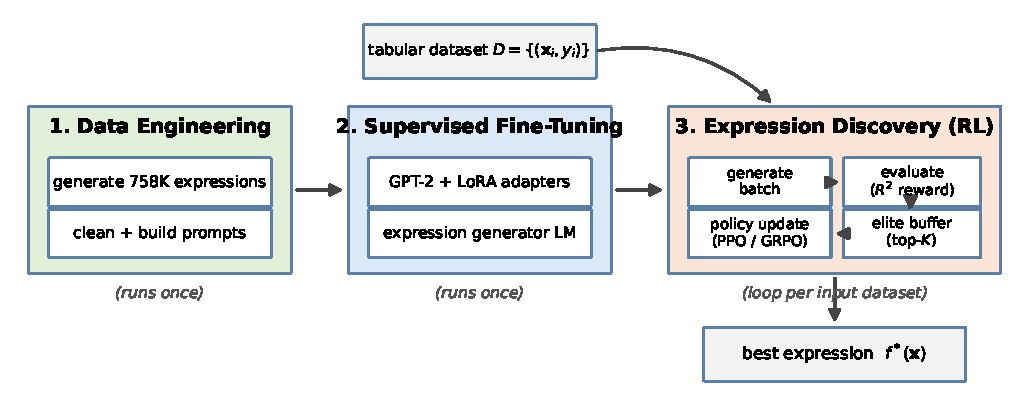
\includegraphics[width=0.98\linewidth]{figures/fig_overview.pdf}
    \caption[End-to-end overview of the Seriguela pipeline]{End-to-end overview of the Seriguela pipeline. Stages 1 and 2 run once and produce a reusable expression-generator model; stage 3 runs per input dataset, optimizing the generator toward the expression that best fits the data.}
    \label{fig:pipeline}
\end{figure}

As illustrated in Figure~\ref{fig:pipeline}, our approach implements a three-stage methodology for symbolic regression:

\begin{enumerate}
    \item \textbf{Data Engineering}: a large corpus of mathematical expressions is generated, validated to remove malformed samples, and formatted into structured training prompts.
    \item \textbf{Supervised Fine-Tuning (SFT)}: a pre-trained language model is specialized on this corpus, turning it into a domain-specific expression generator.
    \item \textbf{Expression Discovery}: the fine-tuned model is optimized with reinforcement learning against a specific tabular dataset, exploring and refining candidate expressions until one fits the data.
\end{enumerate}

The first two stages are executed only once; their cost is amortized over every subsequent problem. Stage 3 restarts for each new input dataset, always from the same SFT checkpoint.

\section{Dataset Engineering}

\begin{figure}[htbp]
    \centering
    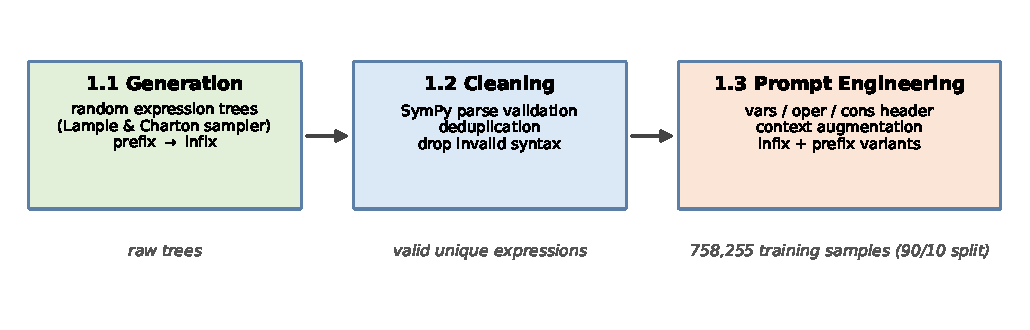
\includegraphics[width=0.98\linewidth]{figures/fig_data_engineering.pdf}
    \caption[Data engineering pipeline]{Data engineering pipeline of the expression corpus: (1.1) random generation of expression trees, (1.2) validation and deduplication, and (1.3) prompt construction.}
    \label{fig:DataEngineering}
\end{figure}

Large language models such as GPT-2 are pre-trained on vast amounts of natural language. Their core objective --- predicting the next most probable token --- is not inherently suited to the syntactically precise, computable language of mathematics. When prompted to produce an equation, a base GPT-2 model typically answers with descriptive text, incorrect formats, or syntactically invalid expressions, as illustrated in Table~\ref{tab:gpt2-comparison}.

To address this limitation, the model is specialized through supervised fine-tuning on a dedicated corpus of mathematical expressions. The data engineering pipeline that builds this corpus consists of three stages --- generation, cleaning, and prompt engineering --- outlined in Figure~\ref{fig:DataEngineering}.

\subsection{Dataset Generation}

\begin{table}[htbp]
    \centering
    \caption{Equation generation configuration parameters.}
    \label{tab:eq_config}
    \begin{tabular}{p{3cm}p{5.2cm}p{4.2cm}}
    \toprule
    \textbf{Parameter} & \textbf{Value} & \textbf{Description} \\
    \midrule
    \texttt{max\_len} & 20 & Maximum token length per equation \\
    \addlinespace
    \texttt{operators} &
    \texttt{add:10, mul:10, sub:5, div:5, sqrt:4, pow2:4, exp:4, sin:4, cos:4, tan:4, asin:2} &
    Operator sampling weights \\
    \addlinespace
    \texttt{max\_ops} & 5 & Maximum operations per equation \\
    \addlinespace
    \texttt{variables} & \texttt{x\_1, \ldots, x\_10} & Base variables (extensible via the \texttt{x\_n} convention) \\
    \bottomrule
    \end{tabular}
\end{table}

The first step was to generate a large volume of diverse mathematical expressions. Expressions are treated as tree structures in which internal nodes are operators (e.g., $+$, $\sin$, $\times$) and leaves are operands --- variables (e.g., $x_1, x_2$) or constants.

To sample these trees without biasing toward overly simple or overly deep structures, we adopted the algorithm proposed by Lample and Charton \cite{lample2019deep}, which gives different tree shapes a near-uniform probability of being generated. The algorithm handles internal nodes with one child (unary operators such as $\sin$) and two children (binary operators such as $+$). Expressions were first created in prefix notation and then converted to the more common infix format. The generation parameters are listed in Table~\ref{tab:eq_config}.

After cleaning and augmentation, the final corpus contains \textbf{758{,}255 expressions}, split into 682{,}429 training samples (90\%) and 75{,}826 validation samples (10\%). The dataset is publicly available on HuggingFace as \texttt{augustocsc/sintetico\_natural\_prefix\_682k}. Table~\ref{tab:dataset_stats} summarizes its statistics and the representation formats available per expression, and Table~\ref{tab:dataset_examples} shows concrete examples.

\begin{table}[htbp]
    \centering
    \caption{Final dataset statistics and available columns.}
    \label{tab:dataset_stats}
    \begin{tabular}{ll}
    \toprule
    \textbf{Statistic} & \textbf{Value} \\
    \midrule
    Total expressions & 758{,}255 \\
    Training split & 682{,}429 (90\%) \\
    Validation split & 75{,}826 (10\%) \\
    File format & Parquet (143 MB) \\
    \midrule
    \textbf{Column} & \textbf{Description} \\
    \midrule
    \texttt{infix\_expr\_n} & Infix notation (natural variables) \\
    \texttt{prefix\_expr\_n} & Prefix notation (natural variables) \\
    \texttt{i\_prompt\_n} & Complete infix prompt for training \\
    \texttt{p\_prompt\_n\_converted} & Complete prefix prompt for training \\
    \texttt{skeleton} & Expression template with variable wildcards \\
    \bottomrule
    \end{tabular}
\end{table}

\begin{table}[htbp]
    \centering
    \caption{Example expressions from the dataset in different formats.}
    \label{tab:dataset_examples}
    \begin{tabular}{p{2.5cm}p{10cm}}
    \toprule
    \textbf{Format} & \textbf{Example} \\
    \midrule
    Infix & \texttt{x\_1*x\_2 + exp(x\_2)} \\
    Prefix & \texttt{+ * x\_1 x\_2 exp x\_2} \\
    Skeleton & \texttt{V*V + exp(V)} \\
    \midrule
    Infix & \texttt{cos(x\_1 + C*x\_2)/sin(C*(C*x\_1 + C)**2)} \\
    Prefix & \texttt{/ cos + x\_1 * C x\_2 sin * C ** + * C x\_1 C C} \\
    Skeleton & \texttt{cos(V + C*V)/sin(C*(C*V + C)**C)} \\
    \bottomrule
    \end{tabular}
\end{table}

The corpus covers a comprehensive set of operators, summarized in Table~\ref{tab:operators}: basic arithmetic, trigonometric functions, and transcendental operations. Variables follow the naming convention \texttt{x\_1}, \texttt{x\_2}, \ldots, \texttt{x\_10}, allowing expressions with up to 10 input features, and constants are represented by the placeholder token \texttt{C}, whose treatment during discovery is discussed in Section~\ref{sec:c_protocol}.

\begin{table}[htbp]
    \centering
    \caption{Mathematical operators available in the dataset.}
    \label{tab:operators}
    \begin{tabular}{lll}
    \toprule
    \textbf{Category} & \textbf{Operators} & \textbf{Arity} \\
    \midrule
    Arithmetic & $+$, $-$, $\times$, $\div$, \texttt{**} (power) & Binary \\
    Trigonometric & $\sin$, $\cos$, $\tan$, $\arcsin$ & Unary \\
    Transcendental & $\exp$, $\log$ & Unary \\
    Other & $\sqrt{\cdot}$, $|\cdot|$ (abs) & Unary \\
    \bottomrule
    \end{tabular}
\end{table}

\begin{table}[htbp]
    \centering
    \caption{Comparison of the GPT-2 model's output before and after fine-tuning, demonstrating its improved ability to generate syntactically correct expressions.}
    \label{tab:gpt2-comparison}
    \ttfamily
    \begin{tabularx}{\textwidth}{ >{\RaggedRight}X >{\RaggedRight}X }
    \toprule
    \multicolumn{2}{c}{\textbf{Base Model}} \\
    \midrule
    \textbf{Prompt} & \textbf{Result} \\
    \midrule
    Generate a mathematical expression that represents the kinetic energy of an object with mass m and velocity v.
    &
    For example, if you want to calculate the kinetic energy of a baseball, you can use the following formula: $K=nx$ \\
    \addlinespace
    Write a trigonometric expression involving sine and cosine that simplifies to 1.
    &
    Write a trigonometric expression involving sin and cosine that simplifies to 1. \\
    \addlinespace
    Instruction: Generate a mathematical expression using variables [x\_1, x\_2, x\_3, x\_4], operands [+, -, *, exp], and [C] as a constant. Expression:
    &
    $x_1 = -(x_2 \cdot x_3) + (x_4 \cdot \exp)$ The expression above is a mathematical expression. \\
    \midrule[1pt]
    \multicolumn{2}{c}{\textbf{After Fine-Tuning}} \\
    \midrule
    vars: x\_1, \ldots, x\_9 \newline oper: *, **, +, -, abs, asin, cos, exp, log, sin, sqrt, tan \newline cons: C \newline expr:
    &
    $x_7 + \exp(C \cdot x_2^C) + C$ \\
    \bottomrule
    \end{tabularx}
\end{table}

\subsection{Data Cleaning}

To ensure the corpus's integrity, every expression was validated with a SymPy \cite{sympy} parser, which flags issues such as unbalanced parentheses or dangling operators. Duplicate expressions were removed to maintain uniqueness.

\subsection{Prompt Engineering}
\label{sec:prompt_engineering}

After generation and cleaning, the corpus was still a plain list of valid expressions --- unsuitable for fine-tuning for two reasons. First, bare expressions provide no \emph{guiding structure}: at inference time there would be no contextual prompt through which to steer generation. Second, the generator produces expressions with limited variable diversity (often five or fewer), and nothing teaches the model to cope with context it does not need.

A prompt engineering phase therefore transformed each raw expression into a structured training sample --- human-readable, token-efficient, and explicit about the elements available for generation:

\begin{verbatim}
vars: x_1, x_2, x_3, x_4, x_5, x_6, x_7, x_8, x_9
oper: *, **, +, -, abs, asin, cos, exp, log, sin, sqrt, tan
cons: C
expr: x_7 + exp(C*x_2**C) + C
\end{verbatim}

To enhance robustness, the \texttt{vars:} and \texttt{oper:} lists were intentionally over-provisioned: for each training sample, a random number of additional variables and operators --- beyond those strictly required by the target expression --- were included. This teaches the model to use only a \emph{subset} of the offered elements, mirroring real scenarios where not every feature is relevant. Finally, both the \textbf{infix} (standard) and \textbf{prefix} (Polish) representations were retained, allowing the notation format itself to be studied as a factor.

\section{Supervised Fine-Tuning}
\label{sec:sft_setup}

With the structured corpus prepared, the next stage teaches the pre-trained model to generate syntactically correct, well-formed expressions. For input processing, the original GPT-2 tokenizer was employed without modification, as its vocabulary adequately covers the mathematical symbols and variables in our data. A useful property of this tokenizer is its fine granularity: words like \texttt{asin} decompose into sub-tokens (\texttt{as}, \texttt{in}) and variables like \texttt{x\_1} into (\texttt{x}, \texttt{\_}, \texttt{1}). This sub-word tokenization, illustrated in Figure~\ref{fig:tokenization}, lets the model generalize to variables never seen during training, such as \texttt{x\_99}.

\begin{figure}[htbp]
    \centering
    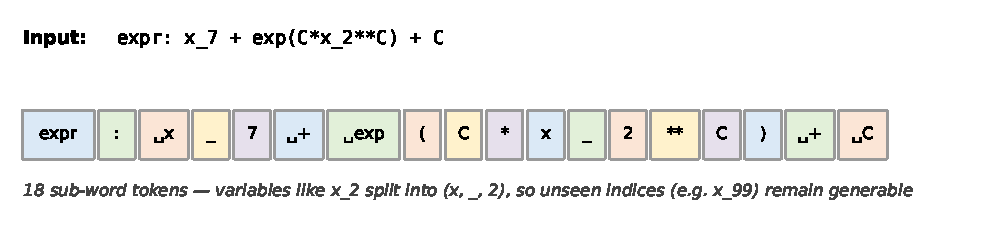
\includegraphics[width=0.95\textwidth]{figures/fig_tokenization.pdf}
    \caption[GPT-2 tokenization of a sample prompt]{GPT-2 tokenization of a sample prompt line. The marker \texttt{␣} denotes a leading space absorbed into the token. Because variables decompose into sub-tokens, unseen indices remain generable.}
    \label{fig:tokenization}
\end{figure}

Fine-tuning used the HuggingFace \texttt{Trainer}. To reduce computational cost and memory usage, we applied Parameter-Efficient Fine-Tuning with LoRA (Section~\ref{sec:bg_finetuning}), targeting the attention projection matrices (\texttt{c\_attn}) of every layer. The key hyperparameters are given in Table~\ref{tab:hyperparameters}. After training, the LoRA adapters were merged into the base weights, and a value head was attached to prepare the model for the PPO arms of the reinforcement learning phase.

\begin{table}[htbp]
\centering
\caption{Hyperparameters for supervised fine-tuning.}
\label{tab:hyperparameters}
\begin{tabularx}{0.82\textwidth}{lX}
\toprule
\textbf{Parameter category} & \textbf{Value / setting} \\
\midrule
\textbf{Optimization} & \\
\quad Optimizer & AdamW (\texttt{adamw\_torch\_fused}) \\
\quad Learning rate & $5 \times 10^{-5}$ with cosine decay (Base); $3\times10^{-5}$ (Medium); $2\times10^{-5}$ (Large) \\
\quad AdamW betas & $\beta_1 = 0.9$, $\beta_2 = 0.999$ \\
\quad Epsilon & $1 \times 10^{-8}$ \\
\quad Weight decay & 0.01 \\
\addlinespace
\textbf{Training} & \\
\quad Epochs & 3 \\
\quad Per-device batch size & 16 \\
\quad Gradient accumulation & 4 (effective batch size: 64) \\
\quad Mixed precision & BF16 \\
\addlinespace
\textbf{LoRA (PEFT)} & \\
\quad Rank ($r$) & 8 (Base); 16 (Medium, Large) \\
\quad Alpha ($\alpha$) & 32 (Base); 64 (Medium, Large) \\
\quad Dropout & 0.05 \\
\quad Target modules & \texttt{c\_attn} \\
\bottomrule
\end{tabularx}
\end{table}

\subsection{Trained Models}
\label{sec:trained_models}

To investigate the effect of model scale and notation format, we trained six model variants covering all combinations of three GPT-2 sizes (Base, Medium, Large) and two notations (Infix, Prefix). Table~\ref{tab:models_trained} summarizes them. All six were fine-tuned on the same 682{,}429-expression corpus with the same schedule (3 epochs; batch size adjusted per model to fit GPU memory); the LoRA rank was increased from 8 to 16 for the Medium and Large models. All models and the dataset are publicly available on HuggingFace for reproducibility.

\begin{table}[htbp]
    \centering
    \caption{Summary of trained models with their configurations.}
    \label{tab:models_trained}
    \begin{tabular}{lllll}
    \toprule
    \textbf{Model} & \textbf{Backbone} & \textbf{Params} & \textbf{LoRA $r$} & \textbf{HuggingFace repository} \\
    \midrule
    Base Infix & GPT-2 & 124M & 8 & \texttt{augustocsc/gpt2\_base\_infix\_682k} \\
    Base Prefix & GPT-2 & 124M & 8 & \texttt{augustocsc/gpt2\_base\_prefix\_682k} \\
    Medium Infix & GPT-2 Medium & 355M & 16 & \texttt{augustocsc/gpt2\_medium\_infix\_682k} \\
    Medium Prefix & GPT-2 Medium & 355M & 16 & \texttt{augustocsc/gpt2\_medium\_prefix\_682k} \\
    Large Infix & GPT-2 Large & 774M & 16 & \texttt{augustocsc/gpt2\_large\_infix\_682k} \\
    Large Prefix & GPT-2 Large & 774M & 16 & \texttt{augustocsc/gpt2\_large\_prefix\_682k} \\
    \bottomrule
    \end{tabular}
\end{table}

\section{Expression Discovery with Reinforcement Learning}
\label{sec:expression_discovery}

Supervised fine-tuning teaches the model the \emph{language} of mathematics, but not the \emph{answer} to any particular problem. To steer the model toward an expression that fits a given dataset, we frame discovery as a reinforcement learning problem, illustrated in Figure~\ref{fig:rl_loop}.

\begin{figure}[htbp]
    \centering
    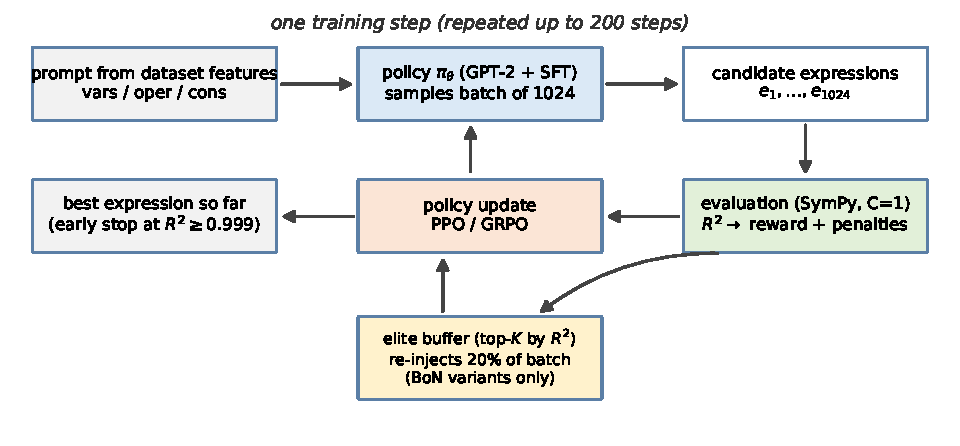
\includegraphics[width=0.92\linewidth]{figures/fig_rl_loop.pdf}
    \caption[The reinforcement learning discovery loop]{One training step of the discovery loop. The policy samples a batch of candidate expressions from the feature-derived prompt; candidates are parsed and scored against the data; the reward drives a PPO or GRPO update. In the BoN variants, an elite buffer retains the best expressions found so far and re-injects them into subsequent batches.}
    \label{fig:rl_loop}
\end{figure}

\subsection{Problem Formulation}

\begin{itemize}
    \item \textbf{State ($s$):} the initial prompt, listing the variables and operators available for the target dataset.
    \item \textbf{Action ($a$):} the autoregressive generation of one complete candidate expression string.
    \item \textbf{Reward ($r$):} a scalar quantifying the quality of the candidate --- primarily its fit to the data --- assigned once the expression is complete (episodic setting, single terminal reward).
\end{itemize}

In practice, discovery begins by loading a tabular dataset and the fine-tuned model. At each step, a batch of 1{,}024 expressions is sampled from the prompt, parsed with SymPy, and evaluated against the training points; the resulting rewards drive one policy update. The loop runs for a fixed budget of 200 steps ($\approx$205K sampled expressions per run) or until an early-stopping criterion fires.

\subsection{The Constant Protocol ($C=1$)}
\label{sec:c_protocol}

The constant token \texttt{C} is instantiated with the fixed value $C=1$ in all training and evaluation runs. This is a deliberate protocol choice: it keeps the reward signal strictly uniform across all algorithmic arms (avoiding the reward confound identified in our preliminary experiments), eliminates the per-expression CPU cost of numerical optimization in the inner RL loop, and is consistent with the zero-shot baselines collected under the same convention. The framework retains an optional constant-fitting routine (L-BFGS-B, bounds $[-2, 2]$), which is reserved for a post-hoc ablation on the champion configuration to quantify the cost of this simplification (Section~\ref{sec:constant_ablation}).

\subsection{Algorithmic Arms}
\label{sec:algorithms}

The experimental core of this work is a controlled comparison of five search strategies, summarized in Table~\ref{tab:rl_algorithms}. All five consume the \emph{same} sampling budget per run, share the same reward, and start from the same SFT checkpoint; they differ only in what they do with the sampled batch.

\begin{table}[htbp]
    \centering
    \caption{The five algorithmic arms compared in this work.}
    \label{tab:rl_algorithms}
    \begin{tabular}{lllll}
    \toprule
    \textbf{Arm} & \textbf{Learning} & \textbf{Advantage} & \textbf{Elite buffer} & \textbf{Value head} \\
    \midrule
    Best-of-N & none (sampling) & --- & no & no \\
    Pure-PPO & policy gradient & EMA baseline & no & yes \\
    Pure-GRPO & policy gradient & group-relative & no & no \\
    BoN-PPO & policy gradient & EMA baseline & \textbf{yes} & yes \\
    BoN-GRPO & policy gradient & group-relative & \textbf{yes} & no \\
    \bottomrule
    \end{tabular}
\end{table}

\subsubsection{Best-of-N Baseline}

Best-of-N draws the full sampling budget from the \emph{frozen} fine-tuned model and returns the highest-scoring expression. No parameter is updated. This baseline measures what the SFT prior alone delivers and is the yardstick for RQ1: any RL arm that fails to beat it, at the same budget, is doing worse than nothing \cite{stiennon2020learning}.

\subsubsection{Pure-PPO}

The PPO arm applies the clipped surrogate objective of Equation~\ref{eq:ppo_clip} to whole-sequence generations, using an exponential-moving-average reward baseline for advantage estimation and a value head attached to the SFT model. Each batch supports up to a fixed number of optimization epochs, with an early stop when the per-epoch KL divergence from the sampling policy exceeds a threshold.

\subsubsection{Pure-GRPO}

The GRPO arm computes advantages by normalizing rewards within groups of samples drawn from the same prompt (Equation~\ref{eq:grpo_adv}, using ranks for scale robustness), requiring no value network. A KL penalty toward the SFT reference model regularizes the update.

\subsubsection{Hybrid Arms: BoN-PPO and BoN-GRPO}

The hybrid arms couple the respective update rule to an \textbf{elite buffer}: a bounded, deduplicated memory of the top-$K$ expressions discovered so far, ranked by $R^2$. During each training step:
\begin{enumerate}
    \item 80\% of the batch is freshly sampled from the current policy;
    \item 20\% is drawn from the elite buffer;
    \item the mixed batch receives the respective update (PPO or GRPO).
\end{enumerate}
The buffer is implemented as a min-heap for efficient top-$K$ maintenance (maximum size 1{,}000, deduplication enabled). Conceptually, it acts as an off-policy anchor in the spirit of Priority Queue Training \cite{petersen2020deep}: rare, high-quality discoveries are converted into a persistent gradient signal instead of being diluted by the next update.

\subsection{Reward Functions}
\label{sec:reward_functions}

Three reward functions were implemented (Table~\ref{tab:reward_functions}). \textbf{R\textsuperscript{2} Clipped} scores pure goodness of fit, clipping the coefficient of determination to $[0,1]$ so that arbitrarily bad expressions cannot dominate the gradient with unbounded negative values. \textbf{Length-Penalized} subtracts a term proportional to expression length ($\alpha = 0.01$ by default). \textbf{SR-IC} is an information-criterion-style reward combining a log-MSE fit term with a complexity penalty, inspired by AIC/BIC-style model selection.

\begin{table}[htbp]
    \centering
    \caption{Implemented reward functions for expression evaluation.}
    \label{tab:reward_functions}
    \begin{tabular}{lll}
    \toprule
    \textbf{Reward} & \textbf{Formula} & \textbf{Purpose} \\
    \midrule
    R\textsuperscript{2} Clipped & $R = \max(0, R^2)$ & pure accuracy \\
    Length-Penalized & $R = \max(0, R^2) - \alpha L$ & accuracy + simplicity \\
    SR-IC & $R = -\log(\text{MSE} + \epsilon) - \lambda C$ & information criterion \\
    \bottomrule
    \end{tabular}
\end{table}

The main experiment uses \textbf{R\textsuperscript{2} Clipped, uniformly across all five arms}. Two considerations forced this choice. First, our preliminary data (Section~\ref{sec:prephase}) contained a reward confound --- BoN arms had been run with SR-IC while pure arms used clipped $R^2$ --- that invalidated any direct comparison; uniformity restores it. Second, and more fundamentally, the pilot study revealed that SR-IC under the $C=1$ protocol has a \emph{dead zone}: its normalization zeroes the reward of nearly every reachable expression, providing no learning signal at all (the empirical demonstration is given in Section~\ref{sec:stability_findings}). Expression complexity is still analyzed --- as a \emph{descriptive} metric of the discovered solutions --- but is not embedded in the training reward.

\subsection{Penalty Strategy for Invalid Expressions}

Sampled strings that fail to parse or evaluate must still receive a learning signal. Two strategies were implemented. The \textbf{binary} strategy assigns every invalid expression the same penalty of $-1.0$. The \textbf{gradient} strategy, used in the main experiment, differentiates by error type, giving the model a smoother path from ``babbling'' to valid mathematics:

\begin{itemize}
    \item Parsing error (invalid syntax): $-1.0$
    \item Variable error (undefined variables): $-0.7$
    \item NaN/Inf error (numerical issues): $-0.5$
    \item Negative $R^2$ (worse than predicting the mean): $-0.3$
    \item Weak fit ($R^2 \in [0, 0.5)$): $0.0$
\end{itemize}

\subsection{Temperature Scheduling}

Sampling temperature controls generation randomness. Three schedules were implemented: fixed ($T = 0.7$), linear annealing, and cosine annealing from $T_{max}=1.0$ to $T_{min}=0.4$. The main experiment uses \textbf{cosine annealing}, allowing broad exploration early in training and progressively sharper exploitation as the run advances.

\subsection{Early Stopping and Stability Guards}
\label{sec:guards}

Four early-stopping criteria bound the cost of each run: (i) \textbf{exact recovery}, $R^2 \geq 0.999$; (ii) \textbf{convergence}, no improvement in best reward within a patience window; (iii) \textbf{policy collapse}, entropy below a threshold indicating mode collapse; and (iv) the hard \textbf{step limit} (200 steps).

Beyond early stopping, the production runs required three engineering safeguards whose necessity was itself an experimental finding (discussed in Section~\ref{sec:stability_findings}): a periodic flush of SymPy's internal caches, which otherwise grow without bound during millions of expression evaluations; a \textbf{complexity cap} that discards pathologically long candidate expressions before symbolic evaluation; and an \textbf{anti-hang watchdog} that times out evaluations of expressions whose simplification stalls the computer-algebra system. The latter two guards were what made the BoN-GRPO arm executable on the harder problems.

\subsection{Fixed Factors and Scope}
\label{sec:fixed_factors}

The framework additionally implements three prompt-conditioning strategies (standard, oracle, and distractor operator lists) and Gaussian noise injection on the target values ($\sigma \in \{0, 1, 5, 10\}\%$ of the target's standard deviation), designed to probe robustness to misleading context and measurement noise. In the final experimental protocol these factors are \textbf{fixed} --- standard prompt, noise 0 --- for two reasons. First, an early large factorial sweep over all factors produced statistically unusable data (Section~\ref{sec:phase_a_lessons}); the redesigned protocol trades breadth for replication, spending the compute budget on five seeds per cell instead of one seed per factor combination. Second, fixing the auxiliary factors keeps the comparison between algorithmic arms strictly interpretable. Robustness to noise and prompt quality remains implemented, documented, and available for future work.

\subsection{Reinforcement Learning Hyperparameters}
\label{sec:rl_hyperparams}

Table~\ref{tab:rl_hyperparams} lists the hyperparameters of the main experiment. One asymmetry deserves emphasis, as it is reported as a finding rather than hidden as a tuning detail: with shared defaults (learning rate $1\times10^{-5}$, 4 PPO epochs, max KL 0.1), the PPO update \emph{destroys} the policy within ten steps --- expression validity falls from 59\% to 0\% and never recovers. The PPO arms therefore use a conservative update (learning rate $1\times10^{-6}$, 2 epochs, max KL 0.02), validated in the pilot study, while the GRPO arms run stably on the defaults. Section~\ref{sec:stability_findings} presents the evidence behind this choice; GRPO on defaults is the \emph{conservative} comparison, since it received no problem-specific tuning.

\begin{table}[htbp]
    \centering
    \caption{Hyperparameters for the reinforcement learning arms (main experiment).}
    \label{tab:rl_hyperparams}
    \begin{tabular}{ll}
    \toprule
    \textbf{Parameter} & \textbf{Value} \\
    \midrule
    \multicolumn{2}{l}{\textit{Common}} \\
    Batch size (expressions/step) & 1{,}024 \\
    Max steps & 200 \\
    Max new tokens & 50 \\
    Temperature schedule & cosine annealing ($1.0 \rightarrow 0.4$) \\
    Reward & R\textsuperscript{2} Clipped (uniform across arms) \\
    Penalty strategy & gradient \\
    Constants & $C=1$ (no fitting) \\
    Entropy coefficient & 0.01 \\
    \midrule
    \multicolumn{2}{l}{\textit{PPO arms (tuned --- see text)}} \\
    Learning rate & $1 \times 10^{-6}$ \\
    PPO epochs per step & 2 \\
    Max KL divergence & 0.02 \\
    Clip $\epsilon$ & 0.2 \\
    \midrule
    \multicolumn{2}{l}{\textit{GRPO arms (defaults)}} \\
    Learning rate & $1 \times 10^{-5}$ \\
    Group size & 8 \\
    KL penalty coefficient & 0.1 \\
    \midrule
    \multicolumn{2}{l}{\textit{Elite buffer (BoN arms)}} \\
    Buffer size & 1{,}000 \\
    Sample ratio & 0.2 \\
    Ranking metric & $R^2$ \\
    \bottomrule
    \end{tabular}
\end{table}

\section{Benchmark Datasets}
\label{sec:benchmarks}

\subsection{Nguyen Suite}

The Nguyen benchmark suite \cite{uy_semantically-based_2011} is a widely adopted collection of twelve symbolic regression problems spanning polynomials, trigonometric compositions, and transcendental functions in one or two variables (Table~\ref{tab:nguyen_benchmarks}). Its problems are small but far from uniform in difficulty: some are solved by virtually any method (saturated), while others --- notably Nguyen-5 --- behave as needles in a haystack, providing the discriminative signal on which the algorithm comparison rests.

\begin{table}[htbp]
    \centering
    \caption{Nguyen benchmark functions.}
    \label{tab:nguyen_benchmarks}
    \begin{tabular}{lll}
    \toprule
    \textbf{ID} & \textbf{Function} & \textbf{Variables} \\
    \midrule
    Nguyen-1 & $x^3 + x^2 + x$ & 1 \\
    Nguyen-2 & $x^4 + x^3 + x^2 + x$ & 1 \\
    Nguyen-3 & $x^5 + x^4 + x^3 + x^2 + x$ & 1 \\
    Nguyen-4 & $x^6 + x^5 + x^4 + x^3 + x^2 + x$ & 1 \\
    Nguyen-5 & $\sin(x^2) \cos(x) - 1$ & 1 \\
    Nguyen-6 & $\sin(x) + \sin(x + x^2)$ & 1 \\
    Nguyen-7 & $\log(x + 1) + \log(x^2 + 1)$ & 1 \\
    Nguyen-8 & $\sqrt{x}$ & 1 \\
    Nguyen-9 & $\sin(x) + \sin(y^2)$ & 2 \\
    Nguyen-10 & $2\sin(x)\cos(y)$ & 2 \\
    Nguyen-11 & $x^y$ & 2 \\
    Nguyen-12 & $x^4 - x^3 + \frac{y^2}{2} - y$ & 2 \\
    \bottomrule
    \end{tabular}
\end{table}

\subsection{SRBench Subset: Feynman and Strogatz}
\label{sec:srbench_data}

For the final challenge phase, we use the ground-truth problems of SRBench \cite{lacava2021contemporary}: the \textbf{Feynman} equations \cite{udrescu_ai_2019} --- physics formulas of one to nine variables --- and the \textbf{Strogatz} suite --- fourteen two-variable systems from nonlinear dynamics. Both are drawn from the PMLB repository \cite{romano2021pmlb}, from which our loaders download data on demand. Combined with the twelve Nguyen problems, the consolidated benchmark of this work comprises \textbf{122 problems} (96 Feynman, 14 Strogatz, 12 Nguyen).

Because the SFT operator vocabulary (Table~\ref{tab:operators}) does not include every function appearing in the physics corpus (e.g., $\arccos$, $\tanh$), each problem is annotated with a \textbf{vocabulary-coverage} flag: for \emph{covered} problems, exact symbolic discovery is possible in principle; for \emph{uncovered} ones, results measure the model's power of \emph{approximation}. Both categories are evaluated and reported --- the distinction is made explicit wherever exact recovery is discussed.

\subsection{Evaluation Protocol and Metrics}
\label{sec:eval_protocol}

Evaluation follows the SRBench ground-truth protocol \cite{lacava2021contemporary}, which we match point by point so that our numbers are comparable with the published leaderboard:
(i) same PMLB datasets;
(ii) 75/25 train/test split;
(iii) $R^2$ reported on the held-out test set;
(iv) evaluation in the zero-noise regime;
(v) \emph{solution rate} defined by the SRBench criterion (test $R^2 > 0.999$);
(vi) differences in computational budget reported as a limitation rather than adjusted for.

Four metrics are used throughout:
\begin{itemize}
    \item \textbf{Best $R^2$ (train):} the highest coefficient of determination achieved on the training points during a run --- the quantity the RL loop optimizes.
    \item \textbf{Test $R^2$:} the score of the selected expression on the 25\% held-out split --- the quantity that certifies generalization.
    \item \textbf{Valid rate:} the fraction of sampled expressions that parse and evaluate --- a process metric tracked per step.
    \item \textbf{Solution rate:} the fraction of runs (or problems) reaching the SRBench discovery criterion, complemented by a manual symbolic-equivalence check (via SymPy simplification) on the discovered candidates.
\end{itemize}
Expression \textbf{complexity} (token count of the discovered formula) is reported descriptively alongside these metrics.

\section{Phased Experimental Design}
\label{sec:design}

The experiments are organized in four phases, each answering a specific question and feeding the next. This design replaces an earlier, much larger factorial sweep whose results proved statistically unusable --- an experience that shaped the methodological priorities here (replication over breadth; process metrics over final scores; see Section~\ref{sec:phase_a_lessons}).

\paragraph{Phase 1 --- Model selection (zero-shot).} All 122 problems are attempted by Best-of-N sampling (no RL) with $N=512$ per seed and \textbf{10 seeds per problem}, using the Base Infix and Large Infix models. The outcome decides which model carries the RL phases: if Base matches or exceeds Large, the smaller model wins on cost.

\paragraph{Phase 1.5 --- Pilot and scouts.} Short, cheap runs ($\sim$US\$2 total) on a single problem to (a) measure step timing for budget planning, (b) validate the reward choice, and (c) probe update stability. The pilot's findings --- the SR-IC dead zone and the PPO collapse --- redefined the protocol of Phase 2 and are reported as results in their own right (Section~\ref{sec:stability_findings}).

\paragraph{Phase 2 --- Controlled algorithm comparison.} The core experiment: $5$ arms $\times$ $4$ problems $\times$ $5$ seeds $= 100$ seed-runs on the selected model. The problems --- Nguyen-3, 5, 7, and 9 --- were chosen to span difficulty: two expected to saturate (sanity checks), one needle-in-a-haystack (Nguyen-5), and one two-variable problem (Nguyen-9). Nguyen-1 was excluded after preliminary data showed every arm solving it (no discriminative signal). Seeds are fixed at $\{42, 123, 456, 789, 1011\}$; every arm consumes the same budget of $200 \times 1024 \approx 205$K sampled expressions per seed.

\paragraph{Phase 3 --- Statistical analysis.} Per-problem one-way ANOVA over best $R^2$ (5 seeds per arm), Tukey HSD post-hoc tests with adjusted $p$-values, and Cohen's $d$ effect sizes for the significant pairs; process-level analyses (exploration width, validity dynamics); and the selection of the champion \emph{(model, algorithm)} configuration. With $n=5$ per cell, power is limited to large effects ($d \gtrsim 1.5$ for 80\% power) --- adequate here because the separations of interest are of that order; given the bimodality of the PPO arms, exact-discovery rates and non-parametric checks complement the ANOVA.

\paragraph{Phase 4 --- SRBench challenge.} The champion configuration runs on \emph{all} 122 problems --- including the vocabulary-uncovered ones, where it measures approximation --- plus five additional uncovered Feynman problems, with a single seed per problem (42), 200 steps each, under the evaluation protocol of Section~\ref{sec:eval_protocol}. The single-seed design is a deliberate budget trade-off: each result is a point estimate rather than a rate, a limitation carried explicitly into the analysis. Its results feed three deliverables: the per-problem ``mother table'' (Appendix~A), the comparison against published SRBench leaderboard numbers, and the dimensional-generalization analysis (RQ4). Finally, the champion undergoes the constant-fitting ablation of Section~\ref{sec:constant_ablation}.

\section{Implementation Details}

\subsection{Software}

The entire implementation is in \textbf{Python}. Model definition, training, and inference use \textbf{PyTorch}; model loading, tokenization, and fine-tuning use \textbf{HuggingFace Transformers} with \textbf{PEFT} for LoRA. The reinforcement learning algorithms (PPO, GRPO, and the BoN variants) were implemented from scratch in PyTorch, providing step-level control over the training dynamics and instrumentation. Symbolic parsing, validation, and simplification rely on \textbf{SymPy}; data handling on \textbf{NumPy} and \textbf{Pandas}; metrics ($R^2$, MSE) on \textbf{scikit-learn}; and the optional constant-fitting routine on \texttt{scipy.optimize} (L-BFGS-B). Experiment tracking used \textbf{Weights \& Biases} during development; all production results are persisted as versioned JSON files (per-seed, with full per-step histories) in the project repository, which is the primary source for every number reported in this work. A CPU-only smoke test validates the full experiment stack in under a minute and is executed before every deployment.

\subsection{Hardware}

Three environments were used across the project's life cycle. Supervised fine-tuning ran on a cloud node with two AMD EPYC 7513 processors (64 cores), 512~GiB RAM, and one NVIDIA A100 80~GB GPU. The reinforcement learning phases ran on rented community-cloud GPUs (RunPod), primarily NVIDIA RTX 3090 24~GB and A40 48~GB instances, with fp16 inference for generation; a local NVIDIA RTX 3050 6~GB workstation executed validation runs and part of the Phase 4 workload (batch size 1{,}024 fits in 6~GB with fp16). Queue-based orchestration --- a YAML experiment queue consumed by a daemon on each machine --- kept all environments running the same code and writing results in the same layout.
